\section{Aspect-Boost}
Aspect-Boost is an initial implementation of Aspect Programming on Artela, and it is a framework for any kind of blockchain and modular blockchain execution layer to integrate to enable Aspect Programming on it. With Aspect-Boost, blockchain can support users to develop, deploy and execute Aspect on it. To integrate Aspect-Boost, blockchain nodes need to implement the adaptors of Aspect-Boots.

Aspect-Boots contains the following key components to boost the process of Aspect integration with different blockchains:

\begin{figure}[h]
  \centering
  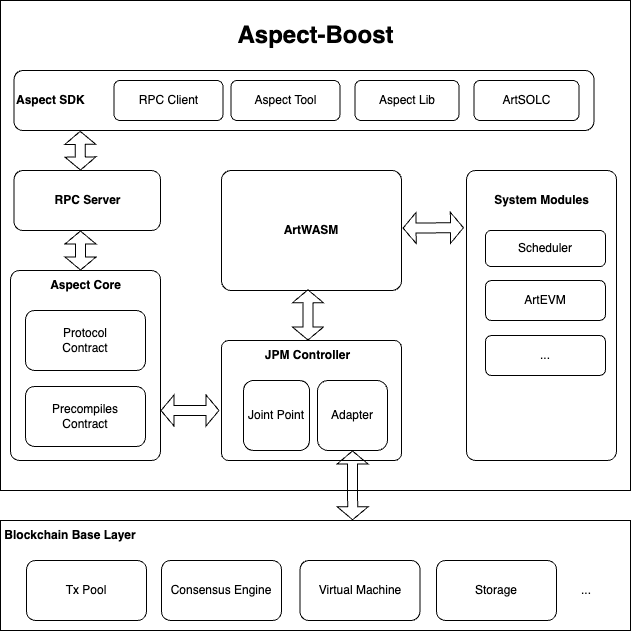
\includegraphics[width=0.4\textwidth]{sections/aspect-boost.png}
  \caption{Aspect-Boost Key Components}
\end{figure}

\begin{itemize}
  \item \textbf{Aspect Core.} The Aspect core is the management module within the Aspect framework and is primarily implemented through smart contracts. It mainly comprises protocol contracts and precompiled contracts. The Aspect core manages major lifecycle processes of Aspects, including deployment, upgrade, and binding, among others. This core module meticulously scrutinizes the ownership of the Aspect in relation to the operation initiator's address, maintains the binding relationships between Aspects and smart contracts, and handles the token settlement for Aspects.
  
  \item \textbf{JPM Controller.} The join point Model controller acts as a hub, connecting the blockchain base layer and the various components of the Aspect framework. It comes into action when specific transaction or block lifecycle stages are reached. Upon the activation of a join point, the JPM controller retrieves the relevant Aspects from the Aspect core, using the address of the smart contract that invoked the action. It then constructs an instance of the Aspect runtime (ArtWASM) to execute the Aspect. In addition, the JPM controller functions as a translator, mediating interactions between the base layer and the Aspect. When an Aspect is invoking base layer functions, the JPM controller's adaptor translates this system call into the corresponding request compatible with the blockchain platform, ensuring the successful execution of the call.
  
  \item \textbf{ArtWASM.} ArtWASM is a tailored WebAssembly (WASM) runtime specifically built for executing Aspects. Functioning as a sandbox, ArtWASM ensures the secure and efficient execution of Aspects within the blockchain environment. Its design incorporates significant optimizations like low context switching latency and high computation throughput, aligning it with the unique requirements of Aspect execution. ArtWASM serves as a bridge between Aspects, system modules, and the JPM controller by providing a comprehensive suite of runtime APIs. These APIs act as the conduit, enabling the necessary communication between these entities. When an Aspect initiates a system call, ArtWASM routes this call to the appropriate module, thereby facilitating seamless integration and interaction across the different components of the Aspect framework.
  
  \item \textbf{System Modules.} System modules comprise a set of system-level modules that can be seamlessly integrated with the blockchain base layer. These modules enhance the functionalities of dApps, enabling them to utilize the full potential of Aspects.
  
  \item \textbf{RPC Server.} The RPC server provides a set of interfaces that are compatible with existing blockchain platforms. These interfaces facilitate the processing of Aspect operations, ensuring interoperability between different platforms.
  
  \item \textbf{Aspect SDK.} The Aspect SDK equips developers with a set of tools to build rich dApps using Aspects. It simplifies the process of incorporating Aspects into dApps and allows for more advanced and flexible applications.
\end{itemize}